\chapter{Continuous Integration}
Continuous Integration is geregeld door Jenkins, dit is een self-hosted omgeving voor continious integration.
Omdat het project met Maven is gebouwd is het makkelijk om CI ondersteuning toe te voegen.
Het commando "mvn test" draait alle tests in het project, als er iets fout gaat is dit ook meteen in Jenkins zichtbaar.

\begin{figure}[H]
	\centering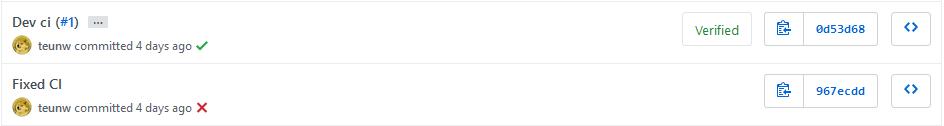
\includegraphics[width=0.35\textwidth]{images/TravisCI.png}
	\caption{Overzicht Jenkins builds}
	\label{fig:jenkins-commits}
\end{figure}
Jenkins wordt geconfigureerd binnen de applicatie zelf, in deze veranderingen staan nu de commando's en Git repoistory geconfigureerd.
Deze configuratie pullt de code vanuit de repository en voert vervolgens het commando "mvn test" uit.
\par
Het bovenstaande script zorgt ervoor dat maven tests automatisch worden uitgevoerd.
De uitslag van deze test is zichtbaar in het build overzicht, zoals in \cref{fig:jenkins-commits} te zien is. Mocht er een build niet succesvol zijn, dan is dit te zien met een rood bolletjes i.p.v. een blauwe.
Jenkins draait je scripts periodiek elke dag, en het resultaat is binnen een paar minuten zichtbaar.

\section{Artifactory}
Nadat Jenkins een build heeft gemaakt wordt deze doorgevoerd naar Artifactory, hier kan de build worden gedownload en ook gedeployed worden op de applicatie server.
Het deployen gebeurt door het WAR bestand weg te schrijven naar een map op de applicatieserver, deze pakt deze vervolgens op en deployed deze.
\begin{figure}[H]
	\centering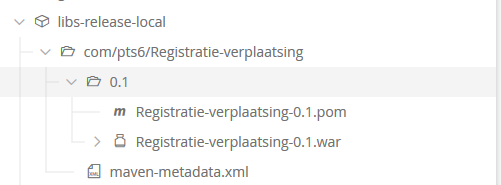
\includegraphics[width=0.6\textwidth]{images/Artifactory_Builds.png}
\end{figure}